\subsection{The software approach} 
\label{sub:the_software_approach}

The pure software approach focuses in improving the \emph{smartness} level of mobile devices by producing software elements that aid them to obtain a better description about the environment and what the user is doing.

As a result, the smartphone can receive key elements that allow it to have a higher level vision of the user activity and to perform informed decisions to adapt its behavior --- sensor usage --- according to the information discovered from context.
In this sense, human activity understanding is based on the discovery of a pattern in the activity and accurate recognition of the activity itself \cite{Yurur2014a}.

All works under this category aim to collect data from sensors and / or other sources of context, process them to obtain information about user activity and employ this information to direct a smarter usage of sensors and other hardware elements of the smartphone.


\subsubsection{Advantages of the software approach}
The pure software approach offers several advantages over the rest of techniques.
Among these advantages are:
\begin{itemize}
  \item There are millions of smart devices already \emph{deployed} around the word, representing a huge infrastructure ready to be used.
  Modify their hardware and in some cases updating the mobile OS\footnote{OS, Operating System.} itself is almost impossible.
  
  \item Although hardware and hardware-software approaches will lead to an undeniable energy saving, their implementations sometimes is very application specific.
  It is due because of the fact that the isolated sensing unit is only capable for being configured for a single mobile app.
  
  \item Current OS's and SDK's\footnote{SDK, Standard Development Kit, the set of compilers, libraries and additional content that allow a programmer to develop applications for that platform (hardware and software).} make it possible to implement a pure-software approach in a logical software unit, such as a middleware or framework.
  This software unit can be embedded in a mobile app just like any other 3rd party library.
  Moreover, it can be installed standalone in the mobile OS and be consumed by mobile apps, in a similar manner the .NET Framework and the Java runtime are installed and utilized.

  \item  By implementing such cognitive processes in the higher software layers, they can be configured, tuned, packed and distributed for their usage in mobile apps running in millions of mobile devices.
  
\end{itemize}

From these points, the most important one is the opportunity to give a smarter behavior to the smartphone and make it participant of higher logical level activities. In this way, the mobile devices are able to detect what the user is doing and how is he/she doing it. Giving this \emph{smartness} opens the path for doing a directed usage of sensors, resulting in energy savings and the adquisition of proper and relevant information.

Based on research in literature, two main branches of the pure software approach has been identified. These branches are described in the next sections.

\subsubsection{Sensors usage adaptation based on user behavior}
\label{ssub:sensors_usage_adaptation_based_on_user_behavior}

It is based on analyzing processes of historical data for detecting patterns in the user behavior.
Once a pattern is detected it is employed to adapt the usage of the sensors.
The new specifications for the sensors usage depends on the purpose of the mobile app framework, however three decisions has been identified.

\subparagraph{Duty cycling}
\label{subp:duty_cycling}
This specific technique tries to adapt the sensor access frequency to reduce energy consumption.
Because of the existence of sleep periods in the sensor being \emph{duty-cycled}, this technique may introduce energy - precision tradeoffs.

In \cite{Perez-Torres2012} a power aware middleware for the support of location and context aware mobile apps with cloud computing interaction is presented.
This middleware incorporate a simple decision rule for determining whether user is in motion. If motion is detected the the GPS continuous readings increment their frequency, otherwise they decrement it.
Through this basic notion of policy authors identified a tendency to obtain energy savings, incrementing the battery life up to 3 times.

\subparagraph{Next value inference}
\label{subp:next_value_inference}
This technique also relies in analysis processes over historical data in order to obtain an approximate inference of the next value that sensors may deliver.

As can be inferred, an actual access to sensor is avoided which may help to reduce energy consumption.
The energy efficiency of this tehcniques depends on the trade-off between the energy consumption of an actual sensor reading against the energy consumed by the computing processes to obtain its inference. Because of this, such technique is useful only when employing high energy consuming sensor or for its use in distributed systems as shown by \cite{Musolesi2010}

\subparagraph{Recycling existing data}
\label{subp:recycling_exsisting_data}
This technique tries to identify common or frequent circumstances or events in contextual information in order to deliver data generated previously.
In this way, an actual access to sensors is also avoided.

In \cite{Chon2014} an energy efficienct mobility monitoring system, FreeTrack, is presented.
This model employs Hidden Markov Models to model the user location inference by collecting data from sources different than GPS.
In this way, the system can identify the place where the user is, for example, employing data coming from cellular and WiFi networks and even from the battery state.

Despite the advantages offered by FreeTrack, a 68\% of energy savings and a precision of 97\% in daily location traces, the main issue is that the system only gives a semantic idea of place as output (e.g. at home, or at work, etc.) instead of location coordinates. 
Because of that there is no way to perform calculations of distance and mobile applications should only use what the system obtains. 
Additionally, FreeTrack may not work if cellular communication is not available or if the user travels constantly since it will begin to miss places frequently.


\subsubsection{Sensor replacement}
\label{ssub:sensor_replacement}

The sensor replacement branch considers the semantic of data in order to find another source of context information.

It refers to consider the purpose of data reading in order to find a different way to obtain the same information. For example, GPS receiver is employed for obtaining the user location but the cellular network data or the wireless networks may also deliver such class of information; even other values like the time of the day and accelerometer data may suggests the location of user.

It is noteworthy the existence of an implicit energy – precision tradeoff due to the changes in the source of context information.
Depending on the relationship of the sensors, there are two types of replacement:

\subparagraph{Directly related replacement}
\label{subp:directly_related_replacement}
The sensor is replaced with another sensor, less energy consuming, that delivers the same type of data without the need of mapping them or additional processing tasks.

In \cite{Lin2010} the A-Loc (adaptive location provider system) is presented.
Based on the accuracy level required by mobile apps, A-Loc chooses the best medium for obtaining user location among GPS, WiFi, cellular tower triangulation and Bluetooth.
% Qué se le critica aquí a A-Loc.

\subparagraph{Context related replacement}
\label{subp:context_related_replacement}

The sensor is replaced with another one that does not deliver the same type of data.
A special process for translating or mapping data is needed for their usage by mobile apps.

In the previous cited work, FreeTrack \cite{Chon2014}, the battery status is employed to determine user location.
Authors consider that users typically charge their smartphones at very well known places, like home or work.
By checking whether battery is charging, the possibilities for deciding user location are dramatically reduced.

However, since the raw data delivered by the new sensor have to be translated, the energy - precision tradeoff is affected heavily: an error in the mapping may bring serious problems.
In the case of FreeTrack, a user charging the smartphone while driving in car causes to obtain wrong results by the software platform.

\subsubsection{Machine learning techniques employed in literature}

In order to detect information about user's context, the mobile app has to employ specific mechanisms to turn the raw data from sensors into information with a significant meaning to the user.

Because of the complexity of human activities and the noise existing in sensor data, the classification algorithm are almost always probabilistic, although machine learning techniques have also been used \cite{Choudhury2008}.

In \cite{Donohoo2014} a description of the most used machine learning techniques is presented. The description of these techniques is summarized in Figure \ref{fig:ml-techniques}.

\begin{figure}
\centering
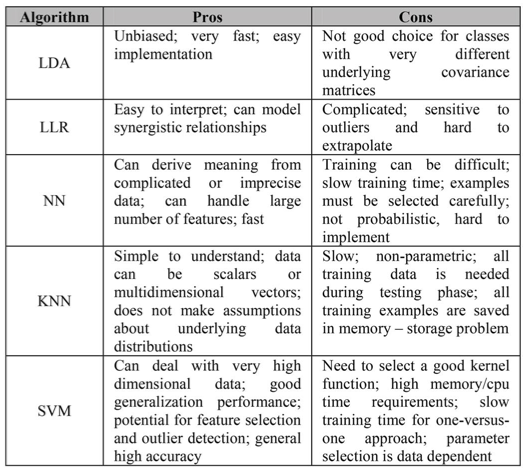
\includegraphics[scale=1.2]{ml-techniques}
\caption[Most used machine learning techniques]{Most used machine learning techniques for modeling user behavior patterns.}
\label{fig:ml-techniques}
\end{figure}

% \begin{itemize}
%   \item Machine learning techniques for determining user behavior

%   \begin{itemize}
%     \item Duty cycling: Adapt the frequenc of use of sensors.
%     \item Next value inference: Infer the next value of the sensor.
%     \item Recycling existing data: From previous information.
%   \end{itemize}

%   \item Sensor replacement: Use less expensive sensors.

%   \item Sensor fusion: Employ different sensors to obtain the data.
%   \begin{itemize}
%     \item Sensors directly related: Several sensors can deliver the same kind of information. For example, location can be obtained via mobile network cell, WiFi and GPS. Use the less expensive sensors.
%     \item Sensors related by contextual information.
%     Even not directly related sensors can be employed to infer the same kind of information. For example, a charging battery, a constant cell ID or static accelerometer data may mean that user is not in motion.
%   \end{itemize}

% \end{itemize}
